\chapter{Anhang}
\section{Pflichtenheft}
\subsection{Projektbeschreibung}

Die Firma ELK wünscht sich ein System mit dem es möglich sein soll,
die Eingangsrechnungen der Lieferanten über eine Internetplattform
zu managen. Die Lieferanten sollen sich anmelden können und so im
Stande sein, ihre Rechnungen als PDF mit Beschlagwortung hochzuladen.
Sobald eine Rechnung hochgeladen wurde, wird die Buchhaltung der Firma
ELK via E-Mail darüber informiert. Die Buchhaltung kann über eine
eigene Internetplattform die Rechnungen herunterladen. Zugestellt
werden sie in Form einer E-Mail, wie diese aussieht, folgt weiter unten.
Die ganzen Vorgänge auf den Plattformen sollen mitprotokolliert werden,
wie zum Beispiel das Löschen einer Rechnung, Holen einer Rechnung oder wenn jemand
eine Benachrichtigung sendet.


\subsection{Zielbestimmungen}


\subsubsection{Muss-Ziele}
\begin{itemize}
\item Lieferantenplattform 

\begin{itemize}
\item Der Lieferant kann sich mit seiner Lieferantennummer registrieren
und wartet bis er vom Administrator freigeschaltet wird. Nach der
Freischaltung erhält er eine Benachrichtigung per E-Mail. 
\item Nur freigeschaltete Lieferanten können sich auf der Plattform anmelden. 
\item Der Lieferant muss angemeldet sein, um Rechnungen hochladen zu können. 
\item Rechnung hochladen: 

\begin{itemize}
\item Rechnungen im PDF-Format hochladen 
\item Beschlagwortung der Rechnungen, vordefinierte Form muss ausgefüllt
werden. Die Vorgaben für die Beschlagwortung werden von der Firma
ELK an uns genauestens übergeben. 
\end{itemize}
\end{itemize}
\item Buchhaltungsplattform: 

\begin{itemize}
\item Es gibt einen gemeinsamen Buchhaltungsbenutzer, wodurch man das Holen
der Rechnungen nicht für die einzelnen Nutzer mitprotokollieren kann. 
\item Wenn der Buchhaltungsbenutzer angemeldet ist, kann dieser: 

\begin{itemize}
\item Rechnungen herunterladen 
\item Rechnungen einsehen 
\item Rechnungen löschen 
\end{itemize}
\item Pro Rechnung wird eine E-Mail versendet. 
\item E-Mail: 

\begin{itemize}
\item Sie enthält die Rechnung als PDF und die Beschlagwortung als XML-Datei,
welche von Herr Ferkl vorgegeben wird. 
\item Dies wird durch einen von uns generierten Job erledigt. 
\end{itemize}
\end{itemize}
\item Administratoransicht: 

\begin{itemize}
\item Der Administrator kann das Intervall festlegen, wann die Passwörter
geändert werden müssen. 

\begin{itemize}
\item Das Intervall kann für Lieferanten und Buchhalter getrennt festgelegt
werden. 
\end{itemize}
\item Der Administrator kann die Lieferanten freischalten sowie auch sperren. 
\item Nur der Administrator kann den Buchhaltungsbenutzer erstellen. 
\item Der Administrator kann \textbf{\small{}KEINE} Rechnungen holen! 
\item Der Administrator kann Kriterien für Passwörter festlegen. Wenn Passwortkriterien
geändert werden, müssen alle Benutzer bei der nächsten Anmeldung ihr
Passwort ändern.
\end{itemize}
\item Loggen: 

\begin{itemize}
\item Lieferanten: 

\begin{itemize}
\item Wenn ein Lieferant eine Rechnung hochlädt 
\item Wenn ein Lieferant einer Rechnung eine Benachrichtigung hinzufügt. 
\item Ob eine Benachrichtigung hinzugefügt oder eine Rechnung hochgeladen
wird, wird jeweils in einer eigenen Logdatei mitgeschrieben. 
\item Ein Eintrag in der Logdatei sieht so aus: {[}Datum{]}-{[}Uhrzeit{]}-{[}Lieferantnummer{]}-{[}Rechnungsnummer{]} 
\end{itemize}
\item Buchhaltung: 

\begin{itemize}
\item Wann und welche Rechnung gelöscht oder geholt wird. 
\item Beide Fälle, gelöscht oder geholt, werden in einer eigenen Logdatei
gespeichert. 
\item Ein Eintrag im Log sieht so aus: {[}Datum{]}-{[}Uhrzeit{]}-{[}Rechnungsnummer{]} 
\end{itemize}
\item Lieferant freischalten/sperren: 

\begin{itemize}
\item Wenn ein Lieferant freigeschaltet oder gesperrt wird. 
\item Ein Eintrag im Log sieht so aus: {[}Datum{]}-{[}Uhrzeit{]}-{[}Lieferantennummer{]}-{[}freigeschaltet/gesperrt{]} 
\end{itemize}
\end{itemize}
\end{itemize}

\subsubsection{Optionale-Ziele}
\begin{itemize}
\item Lieferantenplattform: 

\begin{itemize}
\item Lieferant sieht, welche seiner Rechnungen noch nicht geholt wurden,
kann aber diese nicht mehr ändern. 
\item Falls der Lieferant eine fehlerhafte Rechnung hochlädt, kann er die
Buchhaltung durch Drücken eines Benachrichtungsbuttons informieren. 

\begin{itemize}
\item Die Benachrichtigung erfolgt via E-Mail. In der E-Mail stehen die
Rechnungsnummer und eine Beschreibung des Fehlers. 
\item In der Datenbank wird die Beschreibung des Fehlers zur Rechnung hinzugespeichert. 
\item Buchhaltungsplattform: Falls eine Beschreibung hinzugefügt wurde,
wird diese gekennzeichnet und die Buchhaltung kann sich die Beschreibung
des Fehlers durchlesen.
\end{itemize}
\end{itemize}
\end{itemize}

\subsubsection{Nicht-Ziele}
\begin{itemize}
\item Die bestehende automatische Rechnungsverwaltung der Firma ELK soll
nicht verändert werden. 
\item Die Lieferantendatenbank der Firma ELK besteht schon und soll nicht
verändert werden, sondern nur mit unserer Datenbank synchronisiert
werden. 
\item Nach Versenden der E-Mail, welche die Rechnung und die Metadaten enthält,
ist der Aufgabenbereich unserer Diplomarbeit beendet. 
\end{itemize}

\subsection{Produkteinsatz}


\subsubsection{Anwendungsbereich}

Das Endprodukt wird verwendet, um den Rechnungsaustausch zwischen den
Lieferanten und der Firma ELK elektronisch abzuwickeln, um so die Arbeit
der Buchhaltung der Firma ELK zu minimieren.


\subsubsection{Zielgruppen}

Das System wird hauptsächlich von der Buchhaltung und den Lieferanten
verwendet.


\subsubsection{Betriebsbedingungen}
\begin{itemize}
\item Für den Betrieb der Software ist ein Internetzugang für den Lieferanten
sowie für die Buchhaltung der Firma ELK notwendig. 
\item Der Zugriff auf den Webserver, wo die Webseite gespeichert ist und
die Datenbank muss gewährleistet sein. 
\end{itemize}

\subsection{Produktumgebung}


\subsubsection{Software}

Auf dem Zielsystem wird nur ein Browser gebraucht, da die Software
auf einem Server läuft.


\subsubsection{Hardware}

Zur Verwendung unseres Produktes benötigt man einen Webserver und
einen Rechner mit Internetzugang.


\subsubsection{Produktschnittstelle}
\begin{itemize}
\item Das Produkt wird in das bereits vorhandene automatische Rechnungsverwaltungssystem
der Firma ELK eingegliedert. 
\item Unser Produkt erhält täglich die Lieferantenstammdaten des bereits
bestehenden Oracle Datenbanksystems der Firma ELK. 
\end{itemize}

\subsection{Produktfunktionen}


\subsubsection{Lieferantenansicht}
\begin{enumerate}
\item Der Lieferant registriert sich. 
\item Er wartet bis er freigeschaltet wird und wird durch ein E-Mail über
die Freischaltung informiert. 
\item Lieferant kann sich anmelden. 
\item Lieferant kann eine Rechnung nach der anderen hochladen. 
\item Falls eine Rechnung fehlerhaft ist, kann der Lieferant die Buchhaltung
benachrichtigen. 
\item Kann seine offenen Rechnungen ansehen. 
\end{enumerate}

\subsubsection{Buchhaltungsansicht}
\begin{enumerate}
\item Der Buchhaltungsbenutzer kann sich anmelden. 
\item Buchhaltungsbenutzer kann eine Rechnung einsehen. 
\item Buchhaltungsbenutzer kann Rechnungen via E-Mail holen. 
\item Buchhaltungsbenutzer kann Rechnungen löschen. 
\end{enumerate}

\subsubsection{Administratoransicht}
\begin{enumerate}
\item Administrator kann das Intervall für die Passwortänderung für Lieferanten
und Buchhaltungsmitarbeiter getrennt festlegen. 
\item Administrator kann Lieferanten freischalten, sowie sperren. 
\item Der Administrator kann den Buchhaltungsbenutzer erstellen. 
\item Administrator kann Kriterien für das Passwort festlegen. 
\end{enumerate}

\subsection{Benutzeroberfläche}

Das Design sollte dem von der Homepage der Firma ELK (\url{http://www.elk.at},
Stand: September 2015) ähneln.


\subsection{Qualitäts-Zielbestimmungen}
\begin{itemize}
\item Das Produkt sollte für jeden Benutzer nach einer Einschulung verwendbar
sein. 
\item Durch unseren passwortgesicherten Zugang wird sichergestellt, dass
keine privaten Daten der Firma ELK an die Öffentlichkeit gelangen. 
\end{itemize}

\subsection{Globale Testszenarien und Testfälle}
\begin{itemize}
\item Ein Lieferant kann sich ohne Freischaltung nicht anmelden. 
\item Beim Hochladen der Rechnung muss jedes Feld ausgefüllt werden und
eine PDF angehängt sein. 
\item Das Passwort muss den vorgegebenen Kriterien entsprechen. (Sonderzeichen,
Zahlen, Groß-Kleinbuchstaben) 
\item Das Passwort muss nach dem angegebenen Intervall geändert werden. 
\item Nach dem Hochladen einer Rechnung erhält die Buchhaltung eine E-Mail
und die Rechnung wird in der Buchhaltungsansicht angezeigt. 
\item Der von uns generierte Job, welcher die XML erstellt und XML und PDF
per E-Mail versendet, funktioniert einwandfrei. 
\item Unsere E-Mail wird von der automatischen Rechnungsverwaltung angenommen
und weiterverarbeitet 
\item Es sollen Prüfungen sowie Korrekturmöglichkeiten geben, damit bei
einem Absturz keine inkonsistenten Daten weggeschrieben werden. 
\end{itemize}

\subsection{Entwicklungsumgebung}


\subsubsection{Software}
\begin{itemize}
\item Das Produkt wird auf dem Betriebssystem Windows 10 entwickelt. 
\item Das Produkt wird auf Google Chrome und Mozilla Firefox getestet. 
\item Als Entwicklungsumgebung kommt JetBRAINS PhpStorm Version 9.xx zum
Einsatz. 
\item Zum lokalen Testen wird der Apache-Server von XAMPP verwendet mit
der Datenbankumgebung von Oracle. 
\end{itemize}

\subsubsection{Hardware}
\begin{itemize}
\item Zum Entwickeln werden zwei Laptops eingesetzt. 
\end{itemize}

\subsubsection{Entwicklungsschnittstelle}

Die bereits bestehende Datenbank der Firma ELK dient als Schnittstelle
für unsere neu hinzukommende Datenbank.


\subsection{Ergänzungen}

Die zum Entwickeln notwendige Oracle-Lizenz bekommen wir von der Firma
ELK zur Verfügung gestellt. 

\newpage
\subsection{Use-Case-Diagramm}
\begin{figure}[h]
\centering
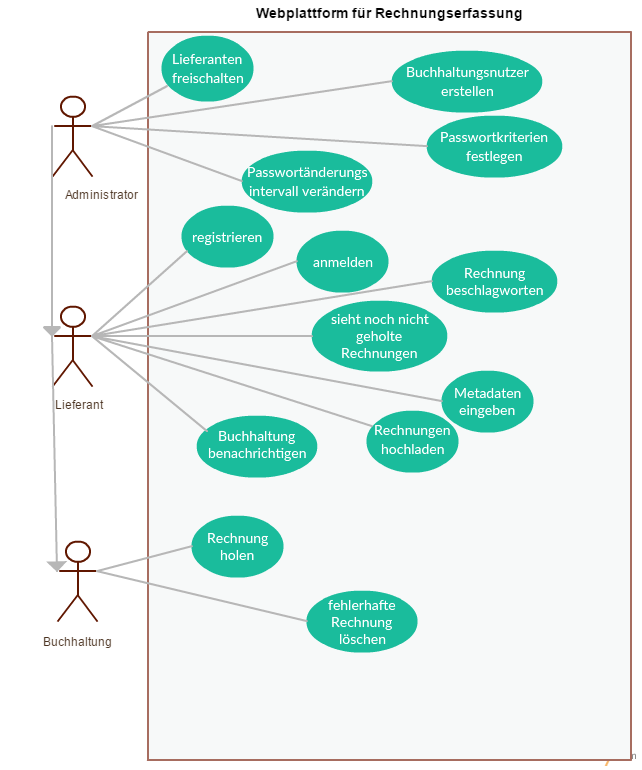
\includegraphics[width=13cm]{figures/Use-Case-Diagramm}
\caption{Use-Case-Diagramm}
\end{figure}

\newpage
\subsection{Quellen}

Dieses Pflichtenheft ist angelehnt an diese Webseite: \\
 \url{http://www.infrasoft.at/downloads/Anleitung_zum_Pflichtenheft.pdf}


\subsection{Unterschriften}

Alle beteiligten Personen sind mit dem Pflichtenheft einverstanden
und das Projekt soll laut diesem Pflichtenheft entstehen. Für weitere
Fragen steht Herr Ferkl zur Verfügung.

\vspace{2cm}

\begin{labeling}{00.00.0000}
\item [{%
\begin{tabular}{>{\raggedright}p{7cm}}
\dotfill{}\tabularnewline
Michael Vogler\tabularnewline
\end{tabular}\hfill{}%
\begin{tabular}{>{\raggedright}p{7cm}}
\dotfill{}\tabularnewline
Florian Mold\tabularnewline
\end{tabular}}]~
\item [{\vspace{2cm}
}]~
\item [{\vspace{2cm}
}]~
\item [{%
\begin{tabular}{>{\raggedright}p{7cm}}
\dotfill{}\tabularnewline
Christopher Ferkl\tabularnewline
\end{tabular}\hfill{}%
\begin{tabular}{>{\raggedright}p{7cm}}
\dotfill{}\tabularnewline
Alexander Mestl\tabularnewline
\end{tabular}}]~\end{labeling}

